\chapter{Generalidades, expresión y purificación de segmentos transmembrana de integrinas $\alpha$IIb/$\beta$3}\label{chap:pept}

Como se mencionó en la introducción (sección  \hl{link a intro}) las integrinas de las subfamilias $\beta$1, $\beta$2 y $\beta$3 juegan un rol muy importante en muchos procesos biológicos relacionados con células epiteliales, endoteliales, leucocitos, fibroplastos y plaquetas, por lo tanto, es relevante obtener información de su estrutura y cómo esta se relaciona con su funcionalidad celular. Para eso es pertinente obtener información acerca de sus interaciones con la membrana lipídica. Uno de los modelos experimentales que nos permite estudiar y comprender las interacciones con lípidos son las capas monomoleculares en interfase agua-aire.

\section{Estructura secundaria de polipéptidos}

La estructura secundaria de los segmentos \ac{tm}-\ac{ic} de la integrina $\alpha$IIb/$\beta$3 (\hl{figura que falta}) se obtuvieron por \ac{rmn} \cite{Yang2009}, además solo unos pocos meses antes Lau Tong-Lay, et al. \cite{Lau2008}, reportaron otra estructura, ambos se realizaron en el sistema de bicelas y se diferencian solo por el largo de unos de los segmentos. La estructura primaria de cada segmento se muestra en la \textbf{figura} \ref{fig:secuencia}, los colores de cada código de letras  \textbf{tabla} \ref{tab:tabla_aa} corresponde a las características fisicoquímicas reflejadas en la \textbf{tabla} ~\ref{tab:percent_hidrofo}; la secuencia va desde el N al C terminal. 
Entre llaves ``\textbf{[ ]}'' se resaltan los residuos que son efectivamente \ac{tm} y al lado izquierdo un pequeño loop \ac{ec} con residuos hidrofóbicos y uno pocos polares que conectan con el dominio \ac{ec} y al lado derecho el dominio \ac{ic} con residuos ácidos y básicos mayoritariamente en ambos péptidos. Para los dos péptidos se observa una alta cantidad de residuos como leucinas (L) y alaninas (A) con tendencia intrínseca de formar estructura secundaria hélice $\alpha$, además de otros residuos hidrofóbicos típicos en proteína transmembrana.

%%%%%Prefencia formar hélice alfa residuos
%%%%%http://facultatciencies.uib.cat/prof/josefa.donoso/campus/modulos/modulo3/modulo3_5_3_1.htm

%\begin{wraptable}{r}{7cm}
%\vspace{-0.5cm} %%%Posiciona a una altura en la hoja
    
\begin{table}[H]   
\centering 
  \caption{Propiedades fisicoquímicas de cada péptido.}\label{tab:percent_hidrofo}
    \begin{tabular}{lcr}

     \toprule  % <-- Toprule here
       & $\alpha$IIb & $\beta$3\\
     \bottomrule % <-- Bottomrule here 

      \textcolor{black}{PM (Da)}            & 6050  & 8762\\
      \textcolor{black}{pI}            		& 4.5  & 4.2\\
      \textcolor{black}{Carga a pH 7.4}            & 4--  & 2+\\
        \textcolor{mygreen}{Hidrofóbicos (\%)}   & 55.56 & 49.37\\
        \textcolor{blue}{Ácidos (\%)}            & 16.67 & 10.13\\
        \textcolor{red}{Básicos (\%)}            & 9.26  & 13.92\\
        \textcolor{black}{Neutros (\%)}          & 18.52 & 26.58\\ % <-- added row here
      \bottomrule % <-- Bottomrule here
      \scriptsize{PM: Peso  molecular}; & \scriptsize{pI: Punto isoelectrico}
    \end{tabular}
    
    \end{table}
%    \vspace{-0.5cm} %%%espacio entre texto y botton table
%    \end{wraptable} 
%%%%%%%%%%%%%%%%%%%%% Fin %%%%%%%%%%%%%%%%%%%%%%%%

%%%%%%%%%%%%%%%%%%%%% Matrix Secuencia %%%%%%%%%%%%%%%%%%%%%%%%
\begin{figure}[H]
    \centering

\begin{minipage}{\textwidth} %
    \resizebox{\textwidth}{!}{

$\begin{NiceMatrix}

\text{$\alpha$}\text{IIb} &   &   &    &    &   &   &    &    &    &  &  &  &  &  & \\
955\text{--}969 & \textcolor{mygreen}{\mathrm{G}} & \textcolor{mygreen}{\mathrm{A}}& \textcolor{mygreen}{\mathrm{M}}& \textcolor{mygreen}{\mathrm{G}}& \textcolor{black}{\mathrm{S}}& \textcolor{red}{\mathrm{E}}& \textcolor{red}{\mathrm{E}}& \textcolor{blue}{\mathrm{R}}& \textcolor{mygreen}{\mathrm{A}} & \textcolor{mygreen}{\mathrm{I}} & \textbf{\Large[} \textcolor{mygreen}{\mathrm{P}} & \textcolor{mygreen}{\mathrm{I}} & \textcolor{mygreen}{\mathrm{W}} & \textcolor{mygreen}{\mathrm{W}} & \textcolor{mygreen}{\mathrm{V}} \\
970\text{--}984 &  \textcolor{mygreen}{\mathrm{L}} & \textcolor{mygreen}{\mathrm{V}} & \textcolor{mygreen}{\mathrm{G}} & \textcolor{mygreen}{\mathrm{V}} & \textcolor{mygreen}{\mathrm{L}} & \textcolor{mygreen}{\mathrm{G}} & \textcolor{mygreen}{\mathrm{G}} & \textcolor{mygreen}{\mathrm{L}} & \textcolor{mygreen}{\mathrm{L}}  & \textcolor{mygreen}{\mathrm{L}} & \textcolor{mygreen}{\mathrm{L}} & \textcolor{black}{\mathrm{T}} & \textcolor{mygreen}{\mathrm{I}} & \textcolor{mygreen}{\mathrm{L}} & \textcolor{mygreen}{\mathrm{V}}\\
985\text{--}999 &  \textcolor{mygreen}{\mathrm{L}} & \textcolor{mygreen}{\mathrm{A}} & \textcolor{mygreen}{\mathrm{M}} & \textcolor{mygreen}{\mathrm{W}} & \textcolor{blue}{\mathrm{K}} & \textcolor{mygreen}{\mathrm{V}} & \textcolor{mygreen}{\mathrm{G}} & \textcolor{mygreen}{\mathrm{F}}\textbf{\Large]} & \textcolor{mygreen}{\mathrm{F}} & \textcolor{blue}{\mathrm{K}} & \textcolor{blue}{\mathrm{R}} & \textcolor{black}{\mathrm{N}} & \textcolor{blue}{\mathrm{R}} & \textcolor{mygreen}{\mathrm{P}} & \textcolor{mygreen}{\mathrm{P}} &\\
1000\text{--}1008  & \textcolor{mygreen}{\mathrm{L}}& \textcolor{red}{\mathrm{E}} & \textcolor{red}{\mathrm{E}} & \textcolor{red}{\mathrm{D}} & \textcolor{red}{\mathrm{D}} & \textcolor{red}{\mathrm{E}} & \textcolor{red}{\mathrm{E}} & \textcolor{mygreen}{\mathrm{G}} & \textcolor{red}{\mathrm{E}} \\

\text{$\beta$}3 \\
684\text{--}698 &    \textcolor{mygreen}{\mathrm{G}} & \textcolor{mygreen}{\mathrm{A}} & \textcolor{mygreen}{\mathrm{M}} & \textcolor{mygreen}{\mathrm{G}} & \textcolor{black}{\mathrm{S}} & \textcolor{blue}{\mathrm{K}} & \textcolor{mygreen}{\mathrm{G}} & \textcolor{mygreen}{\mathrm{P}} & \textcolor{red}{\mathrm{D}} & \textcolor{mygreen}{\mathrm{I}} & \textbf{\Large[}\textcolor{mygreen}{\mathrm{L}} & \textcolor{mygreen}{\mathrm{V}} & \textcolor{mygreen}{\mathrm{V}} & \textcolor{mygreen}{\mathrm{L}} & \textcolor{mygreen}{\mathrm{L}}\\
699\text{--}713  &  \textcolor{black}{\mathrm{S}} & \textcolor{mygreen}{\mathrm{V}} &  \textcolor{mygreen}{\mathrm{M}} & \textcolor{mygreen}{\mathrm{G}} & \textcolor{mygreen}{\mathrm{A}} & \textcolor{mygreen}{\mathrm{I}} & \textcolor{mygreen}{\mathrm{L}} & \textcolor{mygreen}{\mathrm{L}} & \textcolor{mygreen}{\mathrm{I}} & \textcolor{mygreen}{\mathrm{G}} &  \textcolor{mygreen}{\mathrm{L}} & \textcolor{mygreen}{\mathrm{A}} & \textcolor{mygreen}{\mathrm{A}} & \textcolor{mygreen}{\mathrm{L}} & \textcolor{mygreen}{\mathrm{L}}\\
714\text{--}728 & \textcolor{mygreen}{\mathrm{I}} & \textcolor{mygreen}{\mathrm{W}} & \textcolor{blue}{\mathrm{K}} & \textcolor{mygreen}{\mathrm{L}} & \textcolor{mygreen}{\mathrm{L}} & \textcolor{mygreen}{\mathrm{I}} & \textcolor{black}{\mathrm{T}} & \textcolor{mygreen}{\mathrm{I}}\textbf{\Large]} & \textcolor{mygreen}{\mathrm{H}} & \textcolor{red}{\mathrm{D}} & \textcolor{blue}{\mathrm{R}} & \textcolor{blue}{\mathrm{K}} & \textcolor{red}{\mathrm{E}} & \textcolor{mygreen}{\mathrm{F}} & \textcolor{mygreen}{\mathrm{A}} & \\
729\text{--}743 & \textcolor{blue}{\mathrm{K}} & \textcolor{mygreen}{\mathrm{F}} & \textcolor{red}{\mathrm{E}} & \textcolor{red}{\mathrm{E}} & \textcolor{red}{\mathrm{E}} & \textcolor{blue}{\mathrm{R}} & \textcolor{mygreen}{\mathrm{A}} & \textcolor{blue}{\mathrm{R}} & \textcolor{mygreen}{\mathrm{A}} & \textcolor{blue}{\mathrm{K}} & \textcolor{mygreen}{\mathrm{W}} & \textcolor{red}{\mathrm{D}} & \textcolor{black}{\mathrm{T}} & \textcolor{mygreen}{\mathrm{A}} & \textcolor{black}{\mathrm{N}} &  \\
744\text{--}758 & \textcolor{black}{\mathrm{N}} & \textcolor{mygreen}{\mathrm{P}} & \textcolor{mygreen}{\mathrm{L}} & \textcolor{black}{\mathrm{Y}} & \textcolor{blue}{\mathrm{K}} & \textcolor{red}{\mathrm{E}} & \textcolor{mygreen}{\mathrm{A}} & \textcolor{black}{\mathrm{T}} & \textcolor{black}{\mathrm{S}} & \textcolor{black}{\mathrm{T}} & \textcolor{mygreen}{\mathrm{F}} & \textcolor{black}{\mathrm{T}} & \textcolor{black}{\mathrm{N}} & \textcolor{mygreen}{\mathrm{I}} & \textcolor{black}{\mathrm{T}}\\
759\text{--}762 & \textcolor{black}{\mathrm{Y}} & \textcolor{blue}{\mathrm{R}} & \textcolor{mygreen}{\mathrm{G}} & \textcolor{black}{\mathrm{T}} \\

\end{NiceMatrix}$ \\
}
\end{minipage} 

    \caption[Estructura primaria de los segmentos TM-IC de $\alpha$IIb y $\beta$3.]{Estructura primaria de los segmentos \ac{tm}-\ac{ic} de $\alpha$IIb y $\beta$3 (PDB: 2KNC). Los colores de cada letra corresponden a las propiedades fisicoquímicas del residuo, \textcolor{mygreen}{verde: hidrofóbicos (G F I L M V W A P)}, \textcolor{blue}{azul: básicos (R K H (+))}, \textcolor{red}{rojo: ácidos (D E (-))}, \textcolor{black}{negro: otros (S T N Y)}. Datos extraídos de \url{https://www.peptide2.com/N_peptide_hydrophobicity_hydrophilicity.php}.}

    \label{fig:secuencia}
\end{figure}
%%%%%%%%%%%%%%%%%%%%% Fin %%%%%%%%%%%%%%%%%%%%%%%%

La distribución de cargas netas y parciales y la hidrofobicidad de los segmentos de \ac{tm} de integrinas son relevantes par definir las interacciones con la membrana lipídica y particularmente la organización en capas monomoleculares en interfase agua-aire que estudiamos en este trabajo. Se generó un mapa de densidad de carga superficial de los dos péptidos como se muestra en la \textbf{figura} \ref{fig:carga_pept}. Con esta visualización es evidente que los extremos son las regiones polares y con mayor densidad de carga, especialmente el dominio \ac{ic} que interactúa con la fase acuosa en una monocapa. 

%%%%%%%%%%%%%%%%%%%%% Fig Tipo de estruturas de una proteina %%%%%%%%%%%%%%%%%%%%%%%%
\begin{figure}[H] % supposedly places it here ...
    \centering
	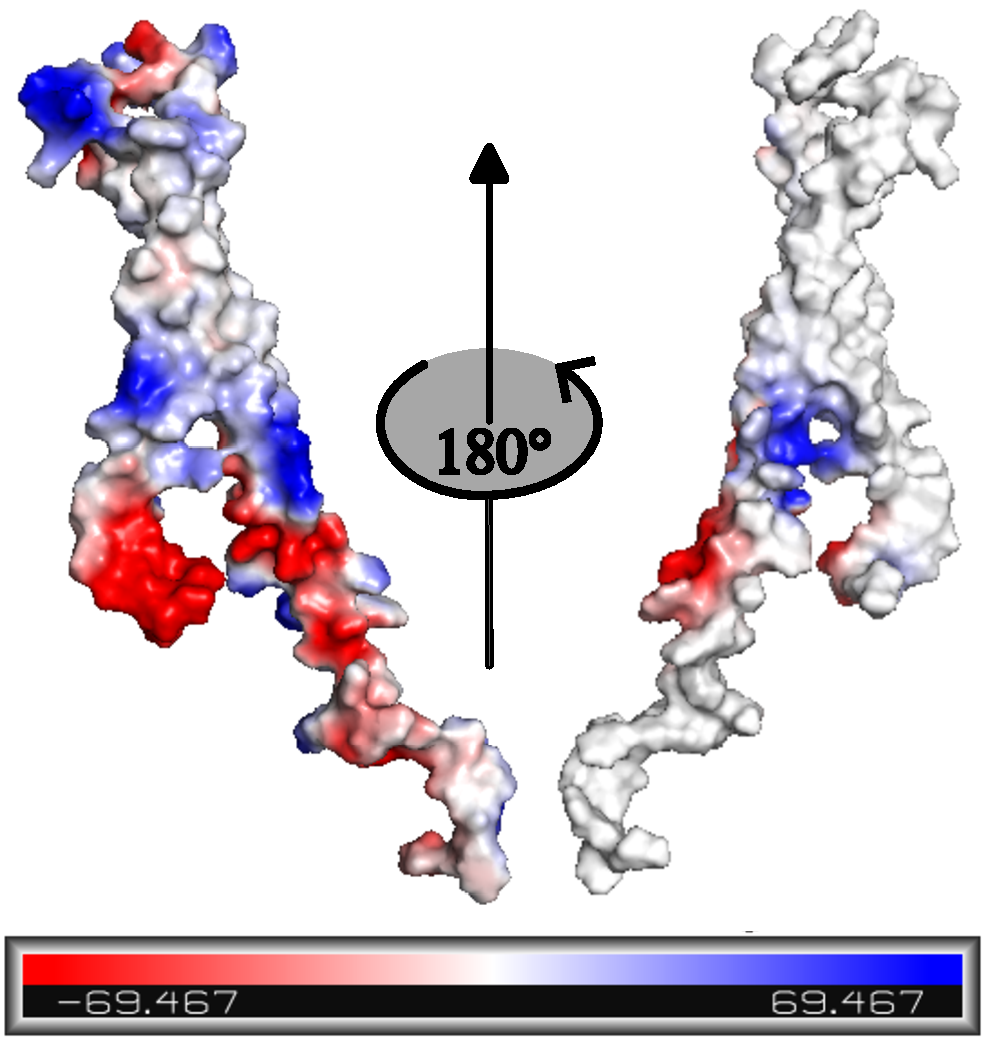
\includegraphics[width=0.79\linewidth]{fig/01_expe/charge_map.pdf}
	\caption[Densidad de carga péptidos]{Densidad de carga péptidos. Los colores corresponden a, \textcolor{red}{rojo: regiones con densidad de carga negativa} y \textcolor{blue}{azul: regiones con densidad de carga positiva}.}
        \index{carga_pept}
    \label{fig:carga_pept}
\end{figure}
%%%%%%%%%%%%%%%%%%%%% Fin %%%%%%%%%%%%%%%%%%%%%%%%

\section{Expresión y purificación de péptidos transmembrana}

La expresión de proteínas por la vía recombinante se ha expandido ampliamente en los últimos años por su versatilidad. Mayoritariamente la obtención de proteínas recombinantes se realiza en células procariotas y la más usada es la bacteria \ac{ecoli} \hl{REF}. El proceso consiste en transformar las bacterias con el plásmido (también conocido como vector) que contiene toda la información genética para expresar la proteína de interés. En este proyecto ambos péptidos se obtuvieron por expresión recombinante empleando bactrias \ac{ecoli} de la cepa BL21(DE3), inducible por \ac{iptg} \hl{REF}. El plásmido empleado para transformar las bacterias fue el pMAL-c2 (ver detalle en la sección \ref{sec:expre_akta}).
Una vez purificada la proteína soluble, que llamamos anteriorme ``proteína fusión'', se clivó con la proteasa \ac{tev} obteniendo la secuencia de los péptidos de interés y posteriorme se repurificaron por \ac{hplc}. 


La \textbf{figura} \ref{fig:expr_hplc_masas}A muestra el seguimiento de la purificación del péptido $\alpha$IIb por \ac{sds}. En los  carriles 1 y 2 se sembró la proteína fusión antes y después del clivaje respectivamente. La pequeña diferencia de peso molecular de $\Xapprox$ 7 kDa, es debida a la ausencia del péptido. En el carril 2 se observa además una banda extra a los $\Xapprox$ 28 kDa que se atribuye a la proteasa \ac{tev}. La banda esperada al péptido no se observa debido a la poca masa que representa. El carril 3 corresponde al pico observado en la cromatografía por \ac{hplc} (\textbf{figura} \ref{fig:expr_hplc_masas}B) que sale en los primeros 6 minutos y se atribuyó a la \ac{mbp}. La banda de peso aparente de $\Xapprox$ 12 kDa en los carriles 4 (fracción directa el HPLC) y 6 (muestra después de retirar \ac{tfa}) corresponden al péptido $\alpha$IIb que corre como dímero debido a su alta hidrofobicidad \hl{REF paper del 2001}. Una vez retirado el \ac{tfa} de las muestras, se realizó un espectro \ac{ftir} en el sistema de \ac{atr} verificando la estructura hélice $\alpha$ mayoritariamente en ambos péptidos, \textbf{figura} \ref{fig:expr_hplc_masas}\textbf{C}. Finalmente la masa molecular de cada péptido fue nuevamente confirmada por espectrometría de masas, resultados que se muestran en la \textbf{figura} \ref{fig:expr_hplc_masas}D-E.

%%%%%%%%%%%%%%%%%%%%% Fig puereza por gel y masas %%%%%%%%%%%%%%%%%%%%%%%%
\begin{figure}[H] % supposedly places it here ...
    \centering
	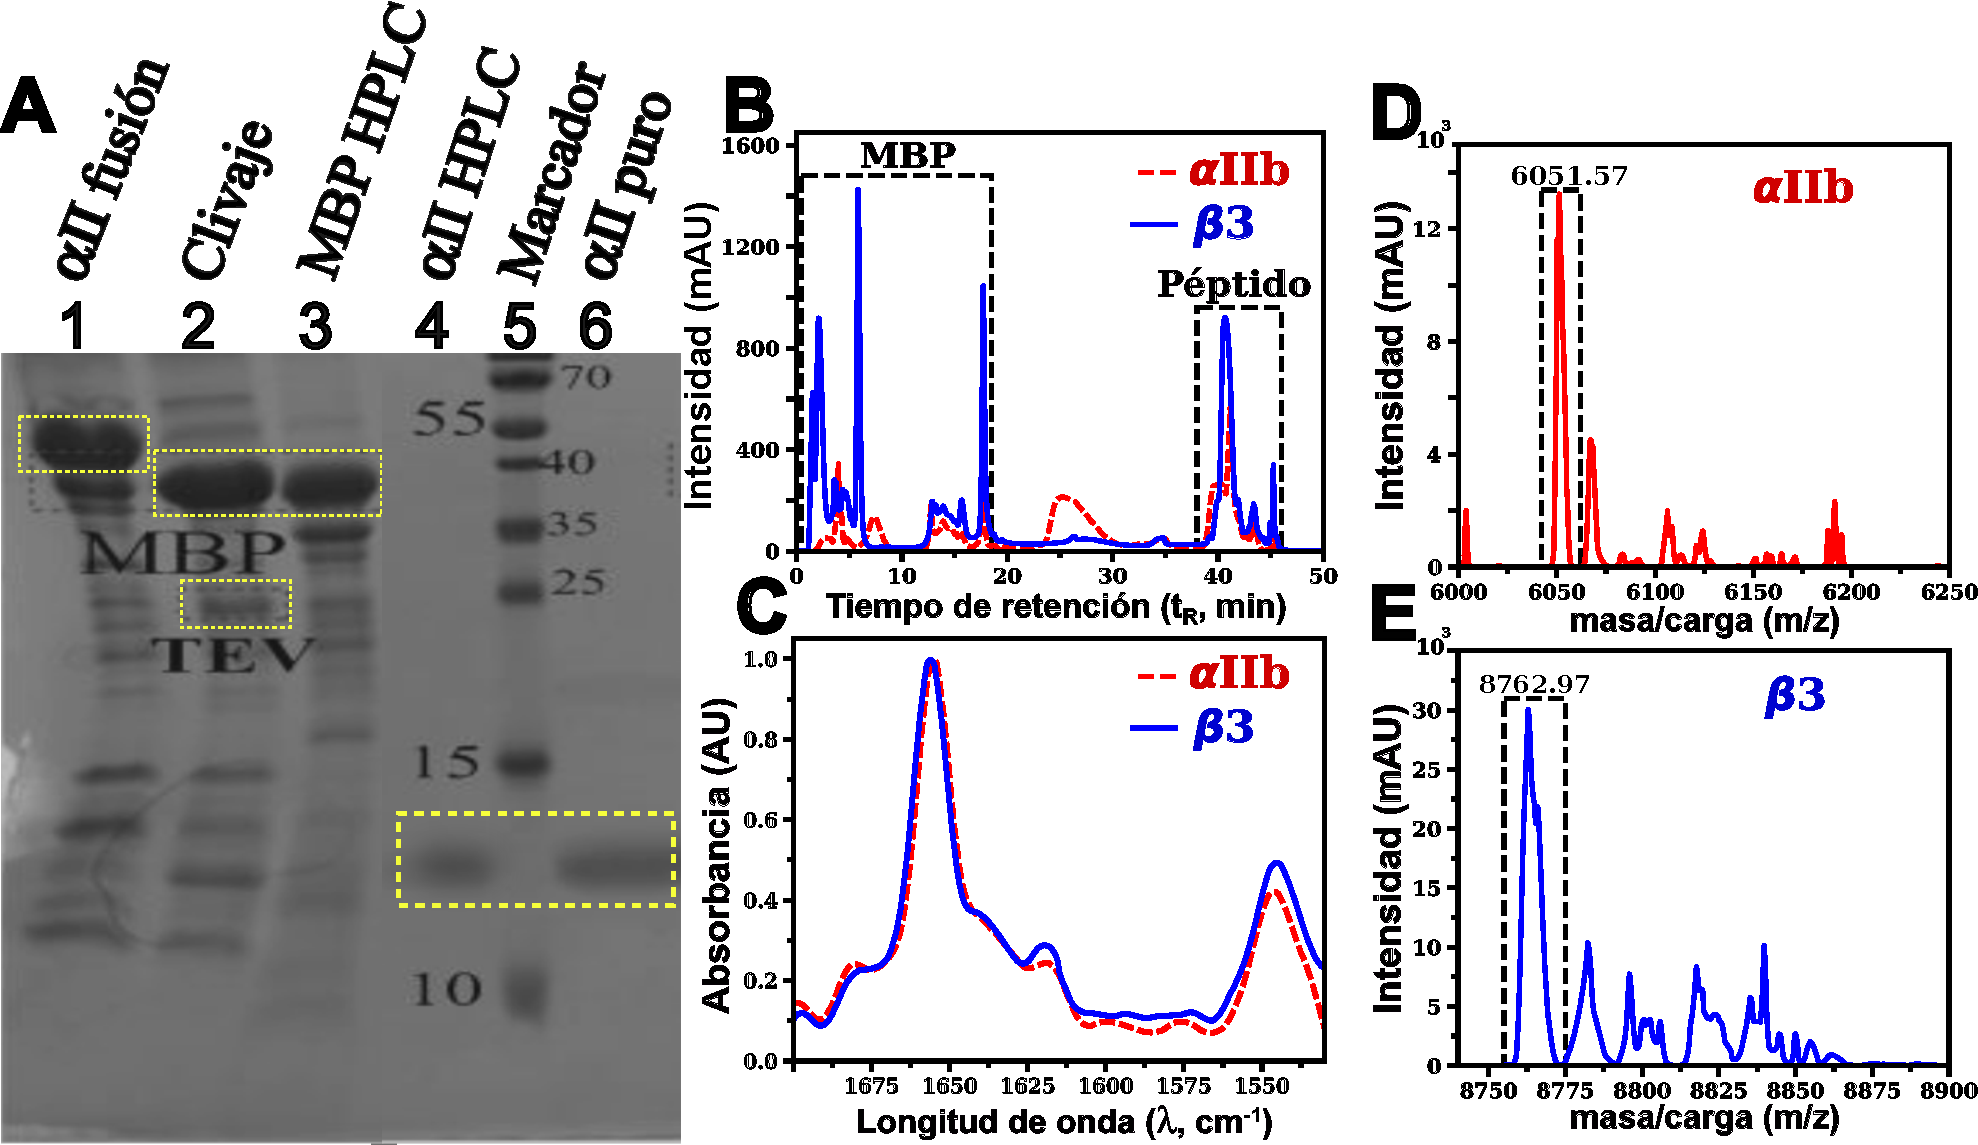
\includegraphics[width=0.99\linewidth]{fig/01_expe/purifi/expres_hplc_masas.pdf}
	\caption[Purificación de péptidos $\alpha$IIb y $\beta$3.]{Purificación de péptidos $\alpha$IIb y $\beta$3. \textbf{A)} Seguimiento de purifición de $\alpha$IIb  por geles \ac{sds}. \textbf{B)} Cromatograma por \ac{hplc} de los péptidos. \textbf{C)} Espectro FT-IR banda de proteína para los dos péptidos y \textbf{D-E)} Espectro de masas para verificación de masa molecular para $\alpha$IIb y $\beta$3 respectivamente.}
        \index{sturcuture_prot}
    \label{fig:expr_hplc_masas}
\end{figure}
%%%%%%%%%%%%%%%%%%%%% Fin %%%%%%%%%%%%%%%%%%%%%%%%





\begin{center} % Center the TikZ picture
\begin{tikzpicture}

% Define box and box title style
\tikzstyle{mybox} = [draw=myblue, fill=blue!10, very thick,
    rectangle, rounded corners, inner sep=10pt, inner ysep=20pt]
\tikzstyle{fancytitle} =[fill=myblue!80, text=white]
\node [mybox] (box){%  
    \begin{minipage}{0.95\textwidth}
    
Las membranas biológicas son un ensamble complejo de una gran variedad de lípidos y proteínas que conjuntamente realizar procesos biológicos importantes a nivel celular. Con la finalidad de entender la funcionalidad de la memebrana, resulta conveniente estudiar las proteínas que son intrínsecamente de membrana. La purificación de proteínas de membrana son un área considerablemente desafiante en la biología molecular \hl{REF}. Un criterio esencial en la purificación de proteínas integrales de membrana es que la proteína debe ser removida cuidadosamente de su ambiente nativo (altamente hidrofóbico) y aislada individualmente en solución. Este solo es posible realizando una secuencia de pasos específicos desde el momento de expresión o síntesis química, de tal forma que en cada paso se recupere la mayor cantidad de la proteína de interés hasta la solubilización con solventes 

%\cite{Carpenter2008}T
%%\cite{Carpenter2008,Eshaghi2009,Matthies2022} \hl{REF}. 

Particularmente en el grupo de investigación del Dr. Guillermo Montich, fue la primera vez que se trabajó con proteínas transmembrana, tampoco había experiencia en el Departamento donde se realizó esta tesis, de otros grupos que hayan expresado y purificado este tipo de proteínas, por lo tanto, una buena parte del tiempo empleado para desarrolar esta tesis consistió en encontrar las condiciones óptimas para la expresión y repurificación los segmentos \ac{tm} de integrimas $\alpha$IIb y $\beta$3. Incluso a modo de anécdota, después de varios intentos sin obtener los péptidos consultamos en laboratorios internacionales que venden el servicio de purificación de proteínas pero después de intercambiar información sobre los péptidos a producir, la respuesta fue que era algo muy complicado y que podría tomar mucho tiempo, buscamos hasta encontrar un laboratorio que tomó el trabajo pero después de dos intentos fallidos nos devolvieron la plata. Queda claro que las proteínas de membrana son desafientes para trabajar, y en el laboratorio hemos desarrollado un protocolo para la obtención de  los segmentos \ac{tm}-\ac{ic} de $\alpha$IIb y $\beta$3 que puede utilizarse para producir estos péptidos y posiblemente péptidos similares. Además, algo que poco se ha mensionado, fue que también se produjo por expresión recombinante la proteasa \ac{tev} que es de venta comercial.

    \end{minipage}
};
\node[fancytitle, right=10pt] at (box.north west) {\Large{Purificación proteínas transmembrana}};
\node[fancytitle, rounded corners] at (box.east) {\faComment };
\end{tikzpicture}%
\end{center}